\chapter{Open Source Power Engineering Software}
\label{sec:oss}
To couple existing implementations of policy gradient reinforcement learning
methods from the PyBrain machine learning library \cite{schaul:2010} with
scalable and extensible optimal power flow formulations, the
Matlab\footnote{Matlab is a registered tradeamark of The Mathworks, Inc.}
source code from \matpower was translated to the Python programming language
for this thesis. With permission from the \matpower developers, the resulting
package was released under the terms of the Apache License version 2.0
\cite{lincoln:pyreto}.  This section briefly describes the project in the
context of other open source Electric Power Engineering software to illustrate the
contribution made.

%\begin{landscape}
%\begin{table}
\begin{sidewaystable}
%\vspace{1ex}
%\begin{small}
\begin{center}
\begin{tabular}{c|c|c|c|c|c|c|c|c|c|c|c|c}
\hline
\textbf{Package} & Language & Licence & PF & DCOPF & ACOPF & CPF & SSSA & TDS &
SE & SP & GUI & RL \\
\hline
AMES & Java & GPL & & \stable & & & & & & & \stable & \stable \\
%Cimphony & Java & LGPL & & & & & & & & & \stable & \\
%CIMTool & Java & LGPL & & & & & & & & & \stable & \\
DCOPFJ & Java & GPL & & \stable & & & & & & & & \\
MatDyn & \matlab & & & & & & & & & \stable & & \\
\matpower & \matlab & & \stable & \stable & \stable & \unstable & & &
\unstable & \stable & & \\
OpenDSS & Pascal & BSD & \stable & & & & & & & \stable & \stable & \\
PSAT & \matlab & GPL & \stable & & \stable &
\stable & \stable & \stable & & \stable & \stable & \\
\pylon & Python & Apache & \stable & \stable & \stable
& & & & \unstable & \stable & \stable & \stable \\
TEFTS & C & & & & & \stable & & \stable & & \stable & & \\
VST & \matlab & & \stable & & & \stable & \stable & \stable & & \stable &
\stable & \\
UWPFLOW & C & & & & & \stable & & & & \stable & & \\
\hline
\end{tabular}
\caption{Open source electric power engineering software feature matrix.}
\label{tbl:featurematrix}
\end{center}
%\end{small}
\end{sidewaystable}
%\end{table}
%\end{landscape}

\section{MATPOWER}
Since 1996, a team of researchers at the Power Systems Engineering Research
Center at Cornell University have been developing \matpower -- a package of
\matlab workspace files for solving power flow and optimal power flow problems
\cite{zimmerman:mp_pes}. Initial development was part of the PowerWeb project
in which the team created a power exchange auction market simulator that could
be accessed by multiple users simultaneously through a web-based interface.
\matpower is available under a custom license that permits it to be used for any
purpose providing the project and authors are cited correctly.  It has become
very popular in education and research and has an active mailing list which is
moderated by Ray Zimmerman.

\matpower includes five power flow solvers for both AC and DC problems.  The
default solver uses Newton's method \cite{tinney:67} with a full Jacobian matrix
updated in each iteration.  Two variations on the fast decoupled method
\cite{stott:74} described in \citeA{amerongen:89} provide quicker convergence
for certain networks.  The standard Gauss-Seidel method \cite{glimn:57} is provided
for academic purposes and the DC solver provides non-iterative
solutions.  The properties of \matlab sparse matrices are fully exploited to
allow the solvers to scale well to very large systems.  All functions are run
from the \matlab command-line or from within users programs and no graphical
user interface is provided.

Starting with version 4.0, \matpower includes the
\matlab Interior Point Solver (MIPS) that can be used for solving
DC and AC optimal power flow problems \cite{zimmerman:ccv}.  Previously,
FMINCON from the \matlab Optimization Toolbox\footnote{Optimization
Toolbox is a registered trademark of The Mathworks, Inc.} was required or one
of a suite of high performance closed-source solvers.  TSPOPF is a
collection of three AC optimal power flow solvers, implemented in the C
programming language and released as \matlab MEX files.  It includes
the original implementation of the step-controlled interior point method from
which MIPS was derived.  MINOPF provides an interface to the
Fortran based MINOS\footnote{MINOS is trademark of Stanford
Business Software, Inc.} solver, developed at the Systems Optimization
Laboratory at Stanford University, and is available only for educational and
research purposes. DC optimal power flow problems can be solved with
a Quadratic Programming interface to MIPS or using a MEX interface to BPMPD --
a commercial interior point method for linear and quadratic programming.

\matpower has an \textit{extensible} optimal power flow formulation that allows
additional optimisation variables and problem constraints to be introduced by
the user.  It is used internally to extend the standard optimisation
formulation to support piecewise linear cost functions, dispatchable loads,
generator PQ capability curves and branch angle difference limit constraints.
Examples of possible additional extensions include: reserve requirements,
environmental costs and contingency constraints.

\matpower currently requires Matlab (version 6.5 or later) which is a
commercial software product from The Mathworks that is supported on all
major platforms.  However, with minimal alteration \matpower has been shown to
run on \textsc{Gnu}/Octave\footnote{\textsc{Gnu}/Octave is an free program for
numerical computation with strong \matlab compatibility.} version 3.2.3.

\section{MATDYN}
\textsc{Matdyn} is an extension to \matpower developed by Stijn Cole from the
Katholieke Universiteit Leuven for dynamic analysis of electric power systems.
It was first released in 2009 under the same license as \matpower and the
same programming style has been used.  The \matpower case format is extended
with structs for dynamic and event data.  \textsc{Matdyn} uses \matpower to obtain a power
flow solution that is then used in solving the system of differential
algebraic equations representing the power system.  Results for \textsc{Matdyn}
are validated against those obtained from PSS/E\footnote{PSS/E is a
registered trademark of Siemens Power Transmission \& Distribution, Inc.~Power
Technologies International.} and the Power System Analysis Toolbox and show
good correspondence.

\section{Power System Analysis Toolbox}
\label{sec:psat}
The Power System Analysis Toolbox (PSAT) is a \matlab toolbox for static and
dynamic analysis of electric power systems developed by Federico Milano,
currently an Assistant Professor at the University of Castilla in Spain. It is
released under the terms of the \textsc{Gnu} General Public License (GPL)
version 2 and offers routines for:
\begin{itemize}
	\item Power flow,
	\item Bifurcation analysis,
	\item Optimal power flow,
	\item Small signal stability analysis,
	\item Time domain simulation and
	\item Phasor measurement unit placement.
\end{itemize}
A large number of input data formats are supported through Perl scripts and
simulation reports can be exported as plain text, Excel spreadsheets or
\LaTeXe~code.  PSAT may be run from the \matlab command-line or through a
\matlab based graphical user interface.  The graphical interface can be used with
Simulink\footnote{Simulink is a registered trademark of The Mathworks, Inc.}
to construct cases such as the network from the UK Generic Distribution System
shown in Figure \ref{fig:ukgds_ehv3}.  A slightly modified version of PSAT that
can be run from the \textsc{Gnu}/Octave command-line is also available.

\begin{figure}
  \centering
  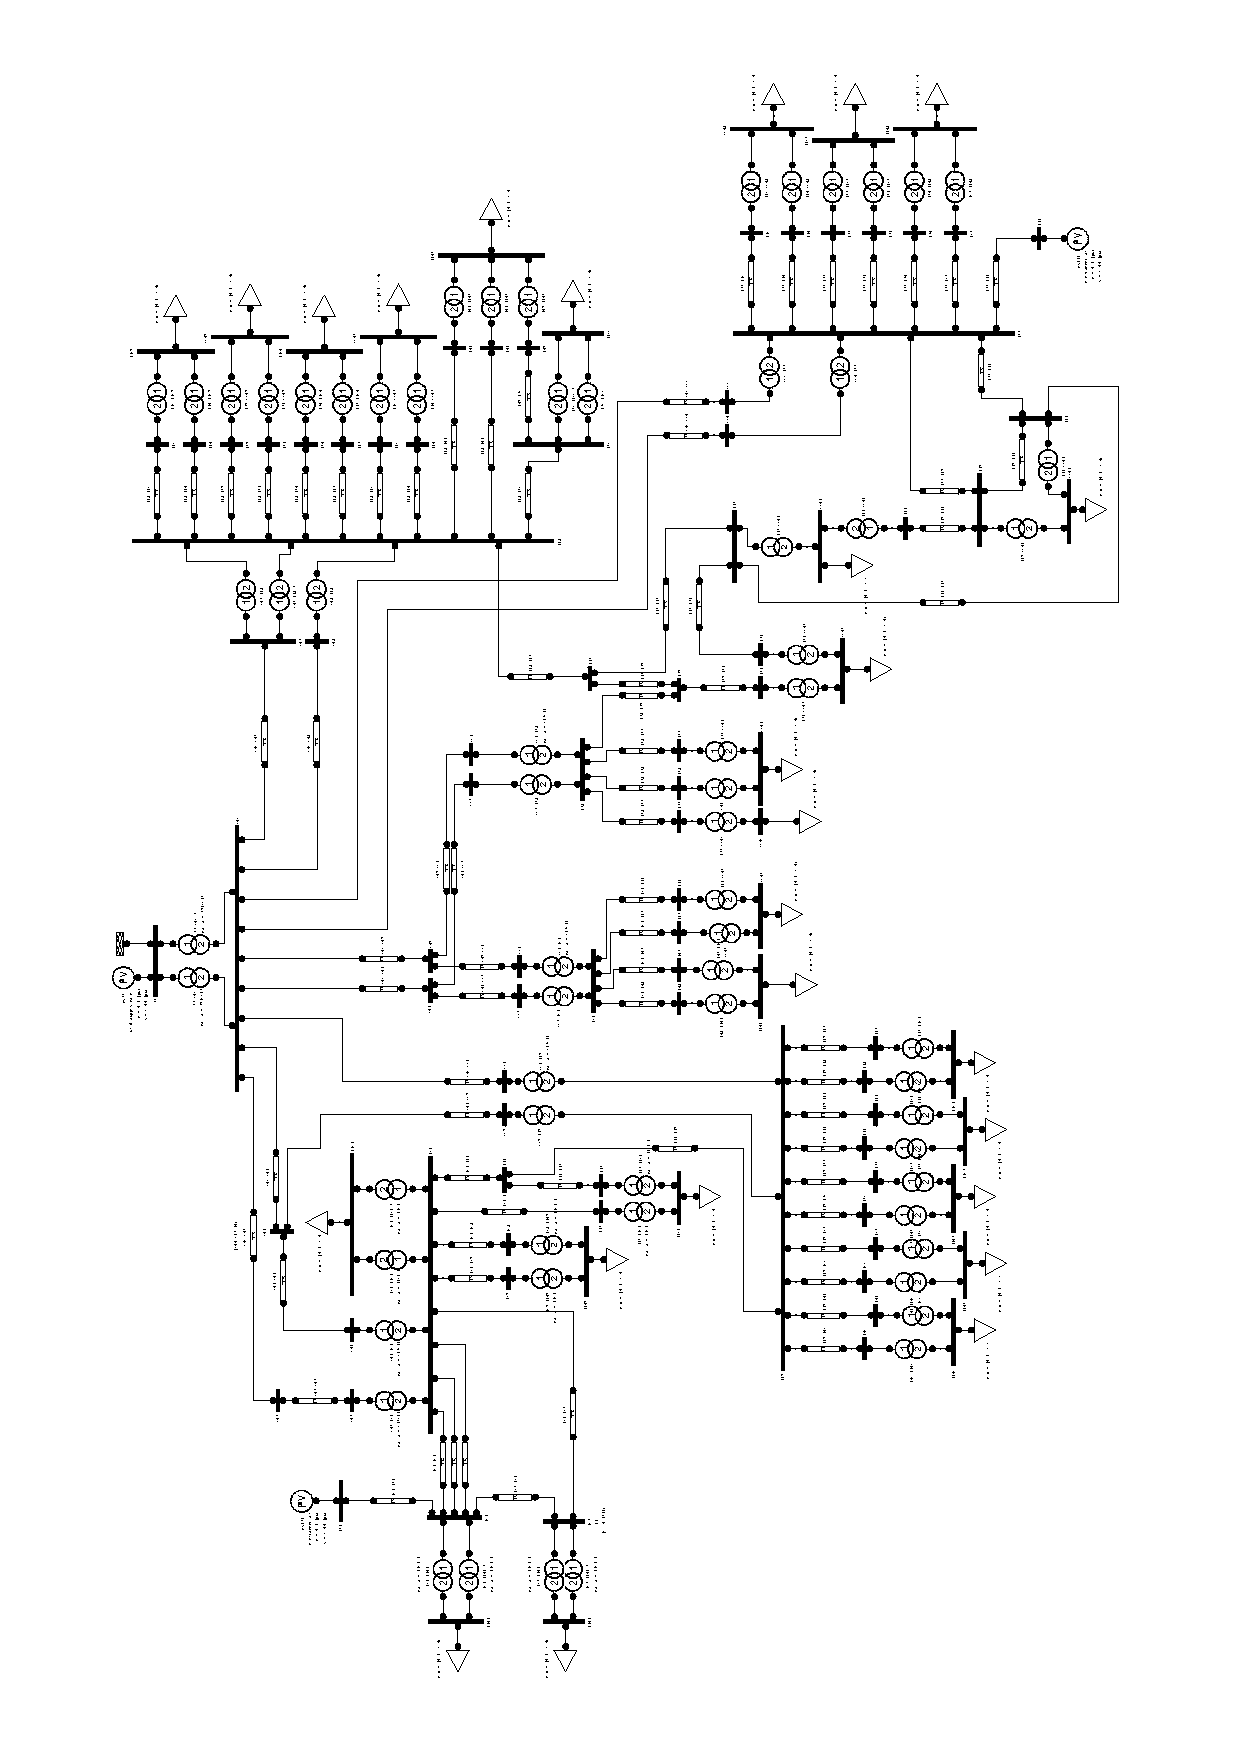
\includegraphics[width=20cm,angle=90]{figures/psat}
  \caption{UKGDS EHV3 model in PSAT Simulink network editor.}
  \label{fig:ukgds_ehv3}
\end{figure}

Optimal power flow problems are solved via an interface to the General
Algebraic Modeling System (GAMS).  GAMS defines optimisation
problems using a high-level modelling language and has a large solver portfolio, including all
of the major commercial and academic solvers.  The interface can be used for
solving single period optimal power flow problems where the objective function
can model maximisation of social benefit, maximisation of the distance to
the maximum loading condition or multi-objective of a combination of these.
Multi-period optimal power flow is formulated as a mixed integer problem with
linearised power balance constraints.  The objective function models
maximisation of social welfare, but is extended to include startup and
shutdown costs.

Power flow and dynamic data are typically separated in electric power
simulation tools, but in PSAT they are integrated.  This combined with the
large number of routines supported by PSAT can make the code base difficult to
understand and modify.  However, comprehensive documentation is included with
PSAT and the mailing list is highly active.
%The majority of correspondance on
%this list concerns PSAT's dynamic simulation features.
The price of GAMS
licenses and the need for optimal power flow problems to be converted to the
GAMS language before being solved could be considered barriers to its
selection for certain projects.

\section{UWPFLOW}
% Continuation and Direct Methods to Locate Fold Bifurcations in AC/DC/FACTS
% Power Systems
UWPFLOW is a research tool for voltage stability analysis developed at the
University of Waterloo, Ontario, and the University of Wisconsin-Madison.  It
is written in ANSI-C and is available as open source for research purposes
only. The program can be run with the terminal command
\begin{center}
\begin{verbatim}
$ uwpflow [-options] input_file
\end{verbatim}
\end{center}
where \texttt{input\_file} is the path to a data file in the IEEE common data
format (CDF) \cite{cdf:73} that may contain High-Voltage Direct Current (HVDC)
and Flexible Alternating Current Transmission System (FACTS) device data.
Output is also in CDF and can include additional data for post-processing,
including values for nose curve plots.  An interface to UWPFLOW is provided
with PSAT and can be used for bifurcation analysis.

\section{TEFTS}
% Transient Stability Program to Study Energy Functions and Voltage Stability
% (Bifurcation) Phenomena in AC/DC Power Systems
The University of Waterloo also hosts TEFTS -- a transient stability program
for studying energy functions and voltage stability phenomena in AC/HVDC
dynamic power system models.  It too is written in ANSI-C and is licensed for
research purposes only.  An executable file for DOS is provided and the source
package contains a simple example.

\section*{Voltage Stability Toolbox}
The Voltage Stability Toolbox (VST) is a \matlab toolbox, developed at the
Center for Electric Power Engineering at Drexel University in Philidelphia, for
investigating stability and bifurcation issues in power systems.  The source
is available for any purpose providing that the authors are suitably cited.
VST features routines for:
\begin{itemize}
  \item Power flow,
  \item Time domain simulation,
  \item Static and dynamic bifurcation analysis,
  \item Singularity analysis and
  \item Eigenvalue analysis.
\end{itemize}
The feature matrix in Table \ref{tbl:featurematrix} shows the similar
capabilities of VST and PSAT. It was developed around the same time and has
the same goals for educational and research applications.  However it does not
have the same quality of documentation nor such an active community of users
and developers as PSAT.

\section{Distribution System Simulator}
In November 2008, the Open Distribution System Simulator (OpenDSS) was released
by the Electric Power Research Institute (EPRI) as open source.  Development of
OpenDSS began in April 1997 and it has been used extensively in distributed
generation impact assessments.  It is the only open source
program designed for both distribution and transmission system simulation.

OpenDSS supports steady-state analysis in the frequency domain, including power
flow, harmonics and dynamics.  Arbitrary $n$-phase unbalanced circuit analysis
is supported using an object orientated data model.  Circuit elements are defined in Object Pascal and solutions are found using a linear sparse matrix solver written in C and
C++.  OpenDSS is available under the Berkeley Software Distribution (BSD)
license, which allows use for almost any purpose.  Circuits are defined in
scripts, using a domain specific language, that may be executed through a
graphical user interface or a Common Object Model (COM) interface.  The user
interface also provides circuit data editing, plotting and power flow
visualisation tools.

The power flow solver is fast and can be configured for repeated
studies using daily, yearly or duty-cycle data.  The multi-phase circuit model allows
complex fault conditions to be defined and three short-circuit analysis methods
are provided.  The heritage of OpenDSS is in harmonics and dynamics analysis
and it does not support system optimisation.

\section{Agent-based Modelling of Electricity Systems}
\label{sec:ames}
The AMES (Agent-based Modeling of Electricity Systems) power market test bed is
a software package that models core features of the Wholesale Power Market
Platform -- a market design proposed by the Federal Energy Regulatory
Commission (FERC) in April 2003 for common adoption in regions of the
U.S.~\cite{tesfatsi:wpmp}. The market design features:
\begin{itemize}
  \item A centralised structure managed by an independent market operator,
  \item Parallel day-ahead and real-time markets and
  \item Locational marginal pricing.
\end{itemize}
Learning agents represent load serving entities or generating companies and
learn using Roth-Erev methods (see Section \ref{sec:rotherev})
implemented with the Repast agent simulation toolkit \cite{gieseler:thesis}.
% The permissive license under which the source code for
% these algorithms has been released allowed direct translation of them for use
% in this study.
Agents learn from the solutions of hourly bid/offer based
DC-OPF problems formulated as quadratic programs using the DCOPFJ package
\cite{tesfatsi:dcopf} described in Section \ref{sec:dcopfj}, below.

The capabilities of AMES are demonstrated using a 5-bus network model in
\citeA{tesfatsi:pes09}.  The model is provided with AMES and a step-by-step
tutorial describes how it may be used.  AMES comes with a
Swing-based graphical user interface with plotting and table editor tools and
is released under the the \textsc{Gnu} GPL version 2.

\section{DCOPFJ}
\label{sec:dcopfj}
To solve market problems defined in AMES, researchers at Iowa State University
developed a stand-alone DC optimal power flow solver in Java named DCOPFJ.
It formulates optimal power flow problems as convex quadratic programs
which are solved using QuadProgJ.  The same researcher developed QuadProgJ as
an independent solver that uses the dual active set strictly convex quadratic
programming algorithm \cite{goldfarb:scqp}.  DCOPFJ requires
generator costs to be modelled as polynomial functions, of second order or
less and no sparse matrix techniques are employed to allow application to large
systems.

\section{PYLON}
\label{sec:pylon}
% Table \ref{tbl:featurematrix} shows that there are open source software tools
% for all of the main Electric Power Engineering problems and that Matlab is the
% most popular language used.  Several of the projects are more than a decade
% old and the relatively recent release of OpenDSS by EPRI shows that interest
% in this approach to development is not fading.

\pylon is a translation of \matpower and Matdyn to the Python programming
language.  It has extensions for agent-based electricity market simulation
that provide features similar to those of AMES.  Both the DC and AC
forumlations of the extensible optimal power flow model \cite{zimmerman:mp_pes}
from \matpower are implemented.  Either a Python version of MIPS or an
interface to the cp solver from CVXOPT can be used to compute solutions.  The
sparsity of the problems is exploited throughout the solution process using
matrix packages from SciPy and bindings to SuperLU or UMFPACK for solver sparse
set of linear equations and performing LU decomposition.  Scripts are provided
for reading and writing data files in PSS/E, \matpower and PSAT format. A wide
variety of learing methods are available in \pylon due to its use of the
PyBrain machine learning library \cite{schaul:2010}.  PyBrain also provides
the artificial neural network models used for policy function approximation
and they may be accelerated using C extension modules from the ARAC project.

In addition to its market simulation capabilities, \pylon also features solvers
for power flow problems (using Newton's method or fast decoupled methods),
state estimation, continuation power flow and time domain simulation.  \pylon
includes a rudimentary GUI that uses the Tkinter library that is included
with Python and thus imposes no additional dependencies.  A more feature
rich GUI is provided by plug-ins for Puddle -- an extensible, GUI
toolkit independant integrated development environment, created for the
purposes of this thesis also.  The use of matrix libraries from NumPy and
SciPy has allowed \pylon (with the permission of the \matpower developers) to
be released under the Apache license, version 2.0. This allows \pylon to be
used in the developement of proprietary software as well as free and open
source software since derivatives of the source code may be made available
under more restrictive terms than the original Apache license.  This is in
contrast to ``copyleft'' licenses, such as the GNU GPL, that require the same
rights to be preserved in modified versions of the work.

% \chapter{PSS/E data for UK Transmission System}
% \section{Power Flow}
% \label{sec:nget_pf}
%
% \section{Optimal Power Flow}
% \label{sec:nget_opf}
